\section{Introduction}
\label{sec:introduction}

The objective of this laboratory assignment is to study a circuit containing:
\begin{itemize}
	\item seven resistors ($R_1$-$R_7$)
	\item one voltage source ($V_a$)
	\item one current source ($I_d$)
	\item one voltage-controlled current source ($I_b$)
	\item one current-controlled voltage source ($V_c$)
\end{itemize}
The circuit is presented in Figure \ref{fig:Desenho_t1}.

In Section \ref{sec:analysis}, a theoretical analysis of the circuit is
presented. In Section \ref{sec:simulation} , the circuit is analysed by simulation,
and the results are compared to the theoretical results obtained in Section
\ref{sec:analysis}. The conclusions of this study are outlined in Section \ref{sec:conclusion}.


\begin{figure}[h]
	\centering
	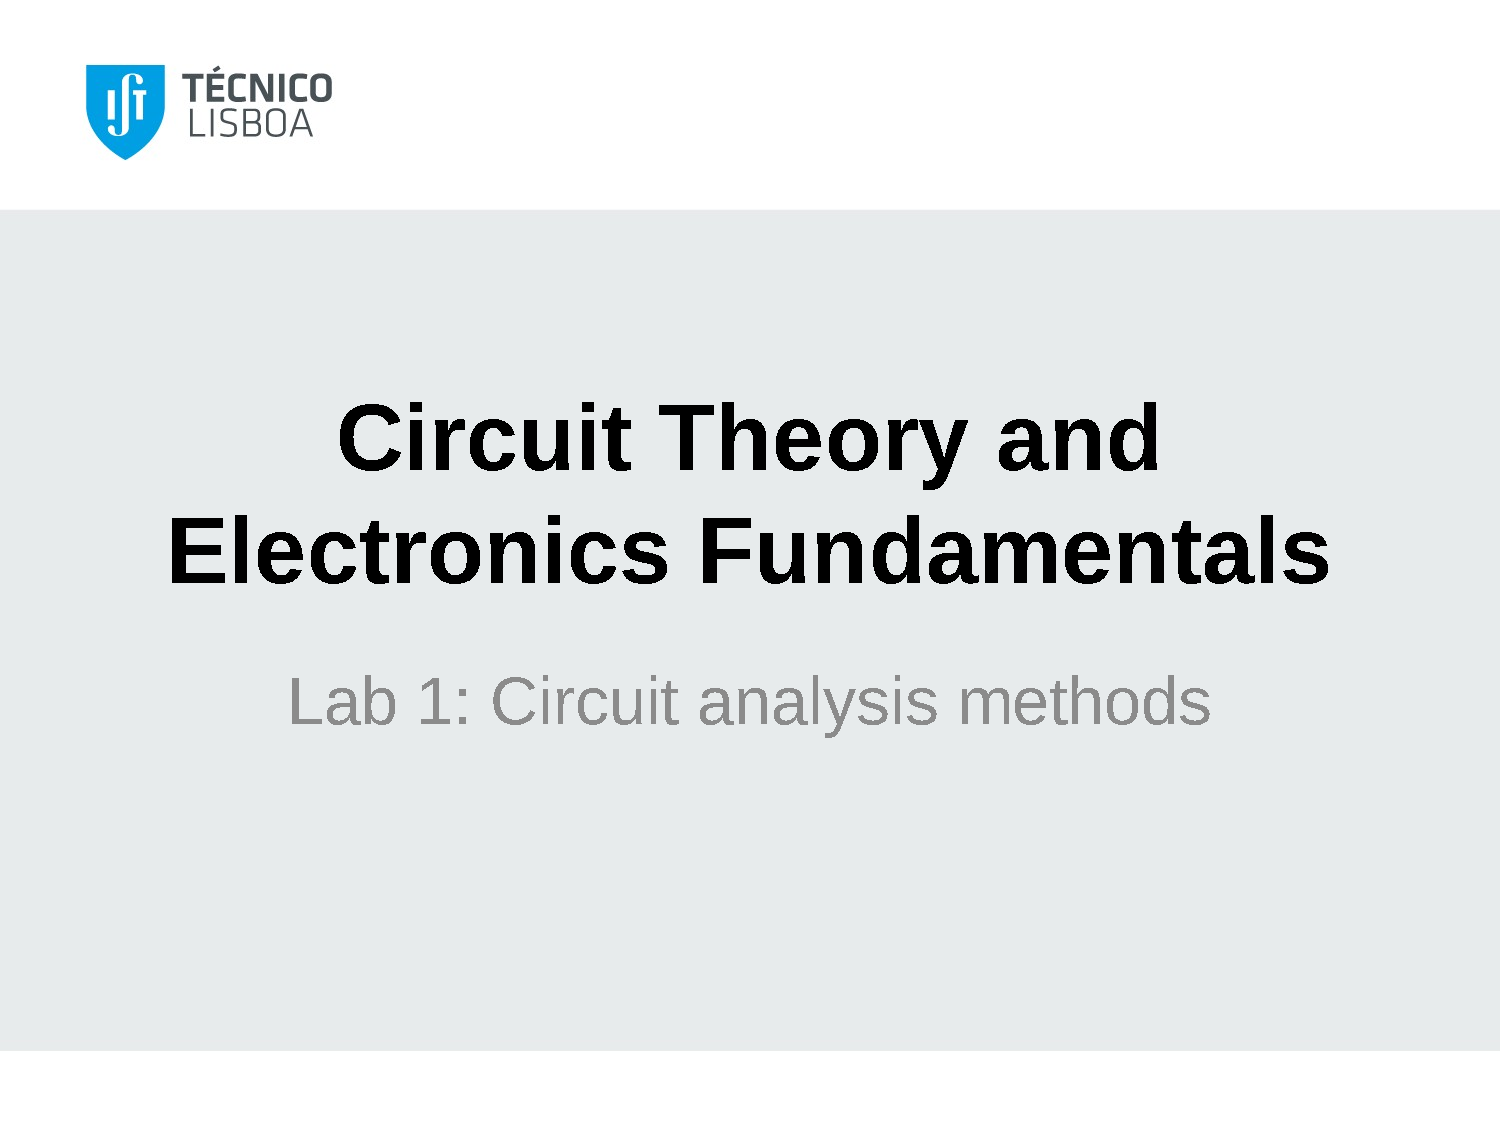
\includegraphics[width=0.85\linewidth]{t1.pdf}
	\caption{Circuit T1}
\label{fig:Desenho_t1}
\end{figure}

